\subsection{Interface}
\label{sect:maw_interface}

\begin{figure}[htb]
    \center{
        % 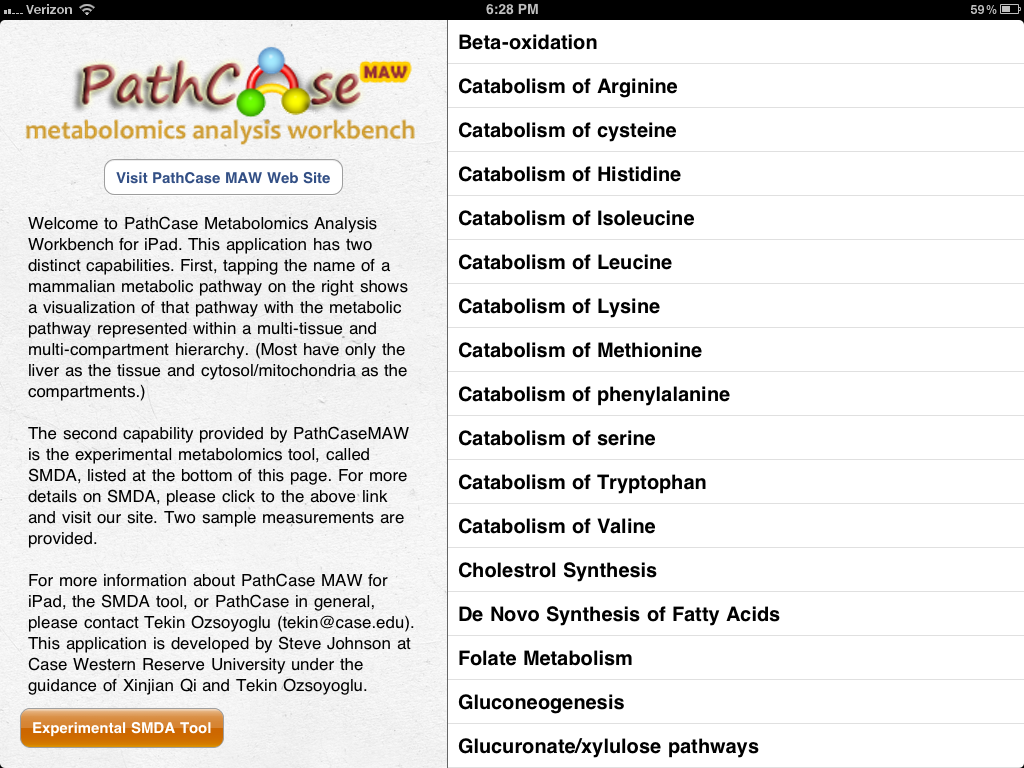
\includegraphics[width=\columnwidth]{maw/figures/screenshot_list}}
        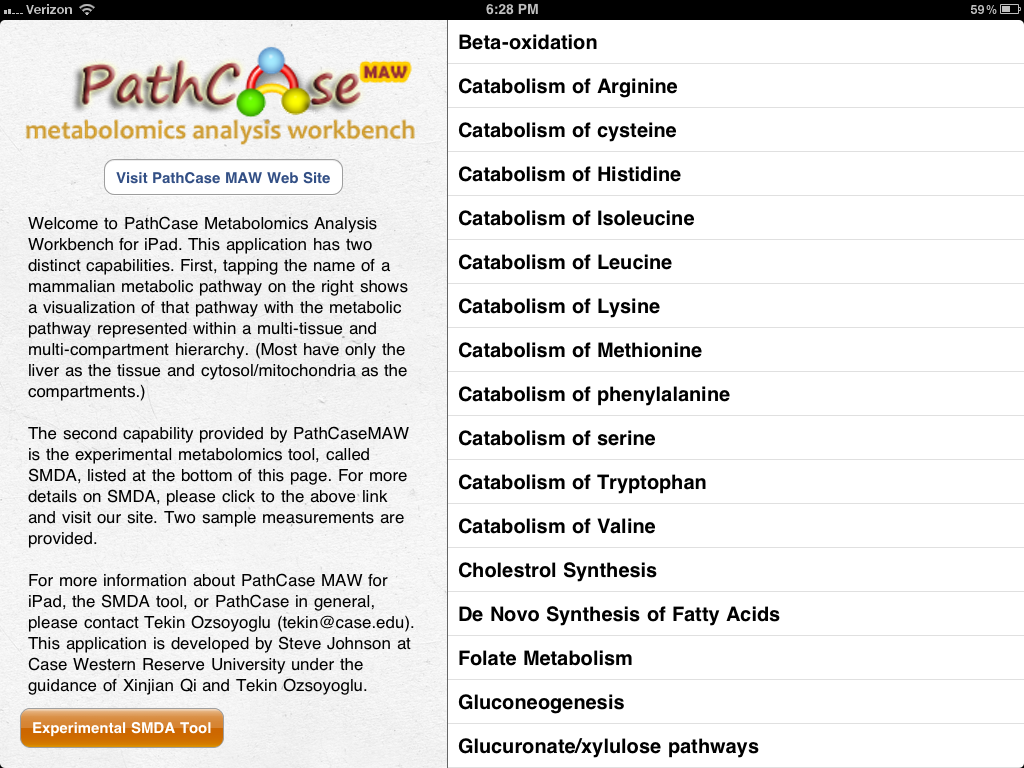
\includegraphics[width=3in]{maw/figures/screenshot_list}}
    \caption{\label{fig:maw_screenshot_list} List of pathways on the main screen
    of \mawapp}
\end{figure}

\begin{figure}[hbt]
    \center{
        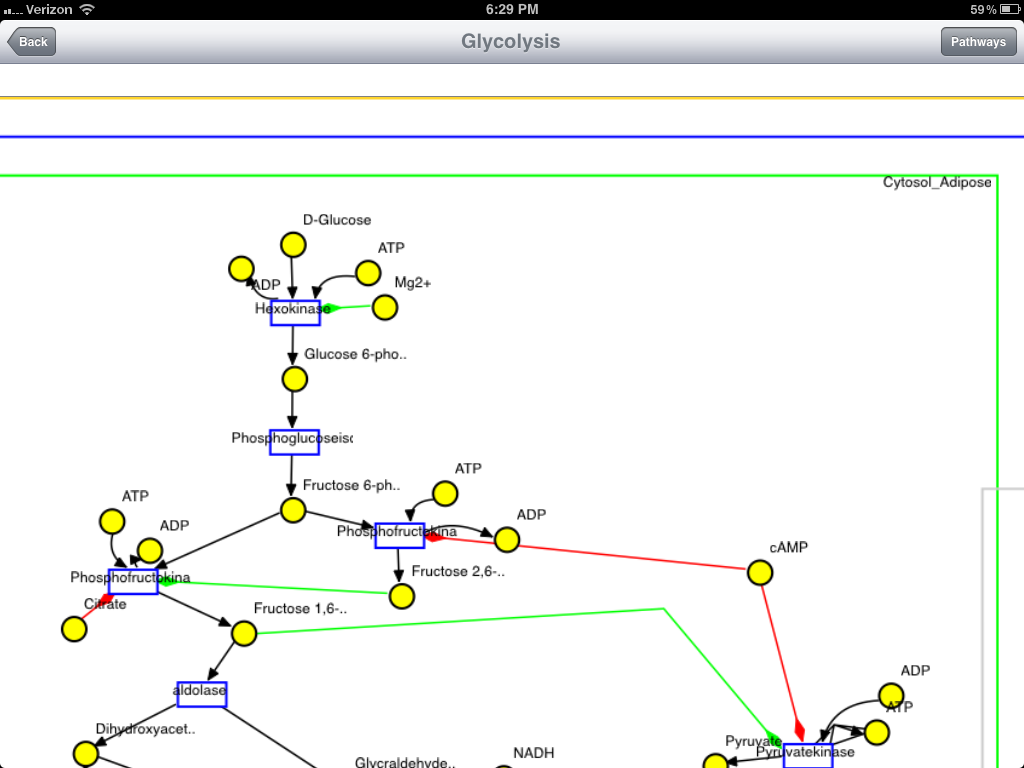
\includegraphics[width=3in]{maw/figures/screenshot_glycolysis}}
    \caption{\label{fig:maw_screenshot_pathway} Scrolling, zooming view of
    Glycolysis}
\end{figure}

The home screen of \mawapp displays a list of pathways that the user can
choose from to view a graph. This screen is shown in figure
\ref{fig:maw_screenshot_list}. It also contains a brief explanation of the
PathCase database and instructions for using \mawapp. The button in the bottom
left corner activates the SMDA part of the app, described in section
\ref{sect:smda}.

After selecting a pathway, the user enters the graph view, where they can pan
and zoom across a pathway. The view for glycolysis is shown in figure
\ref{fig:maw_screenshot_pathway}.

The rectangular nodes of the graph represent processes. The rest of the nodes
represent metabolites. The edges represent relationships such as product,
substrate, cofactor, or inhibitor. The rectangular outlines around sections of
the graph represent the compartment that the pathway is classified under.

When a node is tapped, a popover appears with the full name of the object
represented by the nodes, as well as any relevant relationships or other
information.
